\documentclass[12pt,letter]{article}
\usepackage[margin=1in]{geometry}


\usepackage{amsmath}
\usepackage{amssymb}

\usepackage{graphicx}
\usepackage{hyperref}
%\usepackage{listings}
\usepackage{color}
\usepackage{tabulary}
\usepackage{float}
\restylefloat{table}
\usepackage{indentfirst}


\definecolor{dkgreen}{rgb}{0,0.6,0}
\definecolor{gray}{rgb}{0.5,0.5,0.5}
\definecolor{mauve}{rgb}{0.58,0,0.82}
%
%\lstset{frame=tb,
%  language=Java,
%  aboveskip=3mm,
%  belowskip=3mm,
%  showstringspaces=false,
%  columns=flexible,
%  basicstyle={\small\ttfamily},
%  numbers=none,
%  numberstyle=\tiny\color{gray},
%  keywordstyle=\color{blue},
%  commentstyle=\color{dkgreen},
%  stringstyle=\color{mauve},
%  breaklines=true,
%  breakatwhitespace=true
%  tabsize=3
%}

\begin{document}



\title{Evolving Visual Deception: \\ \large Using a genetic algorithm to generate patterns that confuse motion detection by optic flow algorithms}

\author{Serena Booth, Jacob Peters, Jonathan Bobrow}

\date{March 31st, 2015}
 
\maketitle 
 
\section{Project Description}
We plan to evolve a form of new-age camouflage to disguise motion from optical flow algorithms. 

Visual deception has long been an area of interest for a multitude of reasons, including but not limited to applications of privacy, protection, and fun. Modern day surveillance suggests that privacy is a limited resource and biological systems have evolved unique and robust visual deception techniques. Most of the research and experimentation in this form of crypsis has dealt with static objects and human perception, with the ideal being an invisible cloak (much in the vain of Frodo's); our project, too, will explore solutions for static patterns. However, we aim to conceal motion from optic flow cameras rather than human perception. Because we see examples of counterintuitive camouflage patterns in nature (e.g. a zebra's stripes), we use an evolutionary approach to design static camouflage. 

The question of sensor and algorithm deception has many potential applications. We imagine our system being used to constrain a robot’s area of motion, using a mechanism similar to that of a \href{http://upload.wikimedia.org/wikipedia/commons/6/6b/Lone_Pine,_CA_Virtual_Cattle_Guard.jpg}{virtual cattle guard}. We aim to provide evidence of optical flow being a flawed system for use in traffic navigation by autonomous vehicles. Lastly, we know insects to use optical flow to compute information about flight altitude, amongst other navigation computations, and so we expect our project to equip us with a method of exploiting insect behavior. One example of this may be to design a picnic table which deters insects through a pattern which disrupts optical flow computation.

It is evident that camouflage is useful, and, as such, camouflage from modern sensors and detection algorithms which may now be emphasized more than observation by the naked human eye is a worthwhile area for research. 


\section{Related Prior Work} 

There is increasing interest in the robotics community to implement the optic flow-based navigation strategies used by insects to guide the motion of autonomous robots (Srinivasan 2011a). Insects have a relatively simple, low-resolution, fixed-focus eye structure (the compound eye) which cannot perceive the 3d relationship between features of the environment using stereo vision as vertebrates do (Srinivasan 2011b). However, insects have evolved strategies of determining velocity and relative distance of objects in their environment using motion cues . For example, because nearfield objects produce fast image motion and near field objects produce slow image motion, insects are able to navigate through narrow gaps between vertical objects (i.e., tree branches) by adjusting their position in a way that equalizes the optic flow on the left and right sides of their visual field (Serres et al. 2008, Dyhr and Higgins 2010). Rapid expansion of visual patterns can also indicate that the insect is on a collision course (Tammero and Dickinson 2002). Similar strategies are used to gauge altitude during flight (Egelhaaf 2008, Joesch et al. 2008, Borst 2009), regulate flight speed (Baird et al. 2005, Baird et al. 2010), perform safe landings (Srinivasan et al. 2000), avoid obstacles (Tammero and Dickinson 2002), and coordinate competitive interactions (Land and Collet 1974, Collet and Land 1975 , Boedeker et al. 2003, Collet and Land 1978, Olberg et al 2000). 

Using motion-based cues rather than stereo vision to navigate a three-dimensional environments reduces the computation required to sense and respond to changes in the environment. This advantage is attractive to roboticists building autonomous robots which have limited computation ability and have hardware size/weight constraints, i.e., micro-aerial vehicles (Floreano et al. 2009). Roboticists have successfully implemented insect-inspired motion-based navigation strategies to guide autonomous robots through corridors (Humbert and Hyslop 2010, Srinivasan et al. 2009), perform visual odometry (Chahl and Srinivasan 1996, Weber et al. 1997, Nourani-Vatani et al. 2009), control autonomous aircraft landings (Chahl et al. 2004), and program terrain-following guidance strategies for fixed-wing  and rotary-wing aircraft (Barrows et al. 2003,  Garratt and Chahl 2008). 

Despite the ubiquitous use of motion-based navigation strategies in flying insects and rapidly increasing use of such strategies in robotics, we caution that over-reliance on optic flow makes robots and insects vulnerable to visual deception. In fact, dragonflies have evolved to disguise their motion when hunting by exploiting the weaknesses of optic flow strategies used by their prey (Srinivasan and Davey 1995, Mizutani et al. 2003). Effective optic flow relies on a consistent and predictable environment. Our project aims to evolve static visual patterns that can be used to disguise the motion of objects or deceive a robots optic flow sensors as it navigates through an artificially patterned environment. Our objective is to reveal the limitations of optic flow and introduce the concept of visual deception to increase the stealth of robots and demonstrate that designing unnavigable environments and robot traps for passive defense purposes is feasible. 

Design of visual deception of computer vision algorithms is not unprecedented. A common application of visual deception is digital image encryption. For example, Ragulskis et al. 2007 implemented an algorithm that used stochastic geometric moire patterns to encrypt and decrypt images for file security applications. Recently, deep neural networks (DNN), which use learn hierarchical layers of representation from image data, have been developed to perform human-competitive pattern recognition (Krizhev et al. 2014, Jia et al. 2014). DNNs are used to search image databases and classify image files. Despite the impressive performance of DNNs, Nguyen et al. 2015 used a genetic algorithm to evolve an image that was unrecognizable to a human, but was reported to be a penguin (with 99.99\% confidence) by a state-of-the-art DNN. These deep architectures are thought by many to rival human vision in pattern recognition and classification ability, and yet they can be “easily fooled” using a genetic algorithm. Nguyen et al. used their results as a discussion piece to highlight weaknesses of DNNs. We hope that our study will yield similar results that expose the weaknesses of common optic-flow algorithms and suggest potential applications for fooling enemy optic-flow-dependent robots.

\section{One sentence summary} 

Using a genetic algorithm, we will evolve a form of new-age camouflage which disguises motion as computed by current optic flow algorithms. 

\section{Plan of Execution}

 In order to generate patterns for motion obfuscation, or for specifically targeted optic flow camouflage, we will approach discrete types of motion with generated black and white images. The goal is to produce a pattern that is perceived by an optic flow algorithm as the opposite of its actual movement, so the fitness tests will match this goal. The three discrete tests that we have specified are translational, zoom (approach/retreat), and rotational camouflage. 

To evolve a population of generative patterns, we have set a specific setup as well as testing procedure. The first setup will be a simulation of camera feed tested agains a common optical flow algorithm from OpenCV. Instead of using a webcam or live feed camera, we will feed the optical flow algorithm a 320x240 image generated by the computer and animating our moving target (100x100px) each frame. The background of the image 320x240 will be selected as our possible locations or scenery for camouflage. The 100x100 target will be our object to test and conceal from the optic flow algorithms. 

For translation, the target will travel from one side of the frame to the other, at a fixed speed. The animation will move from left to right (220px of movement) over the course of n-frames, where n $\not=$ 220, since that would provide the virtual camera a perfect image (not representative of an actual camera with a scanning rate). Diagrams for the tests are attached (Figures 1, 2, and 3).

\begin{figure}[H]
    \centering
    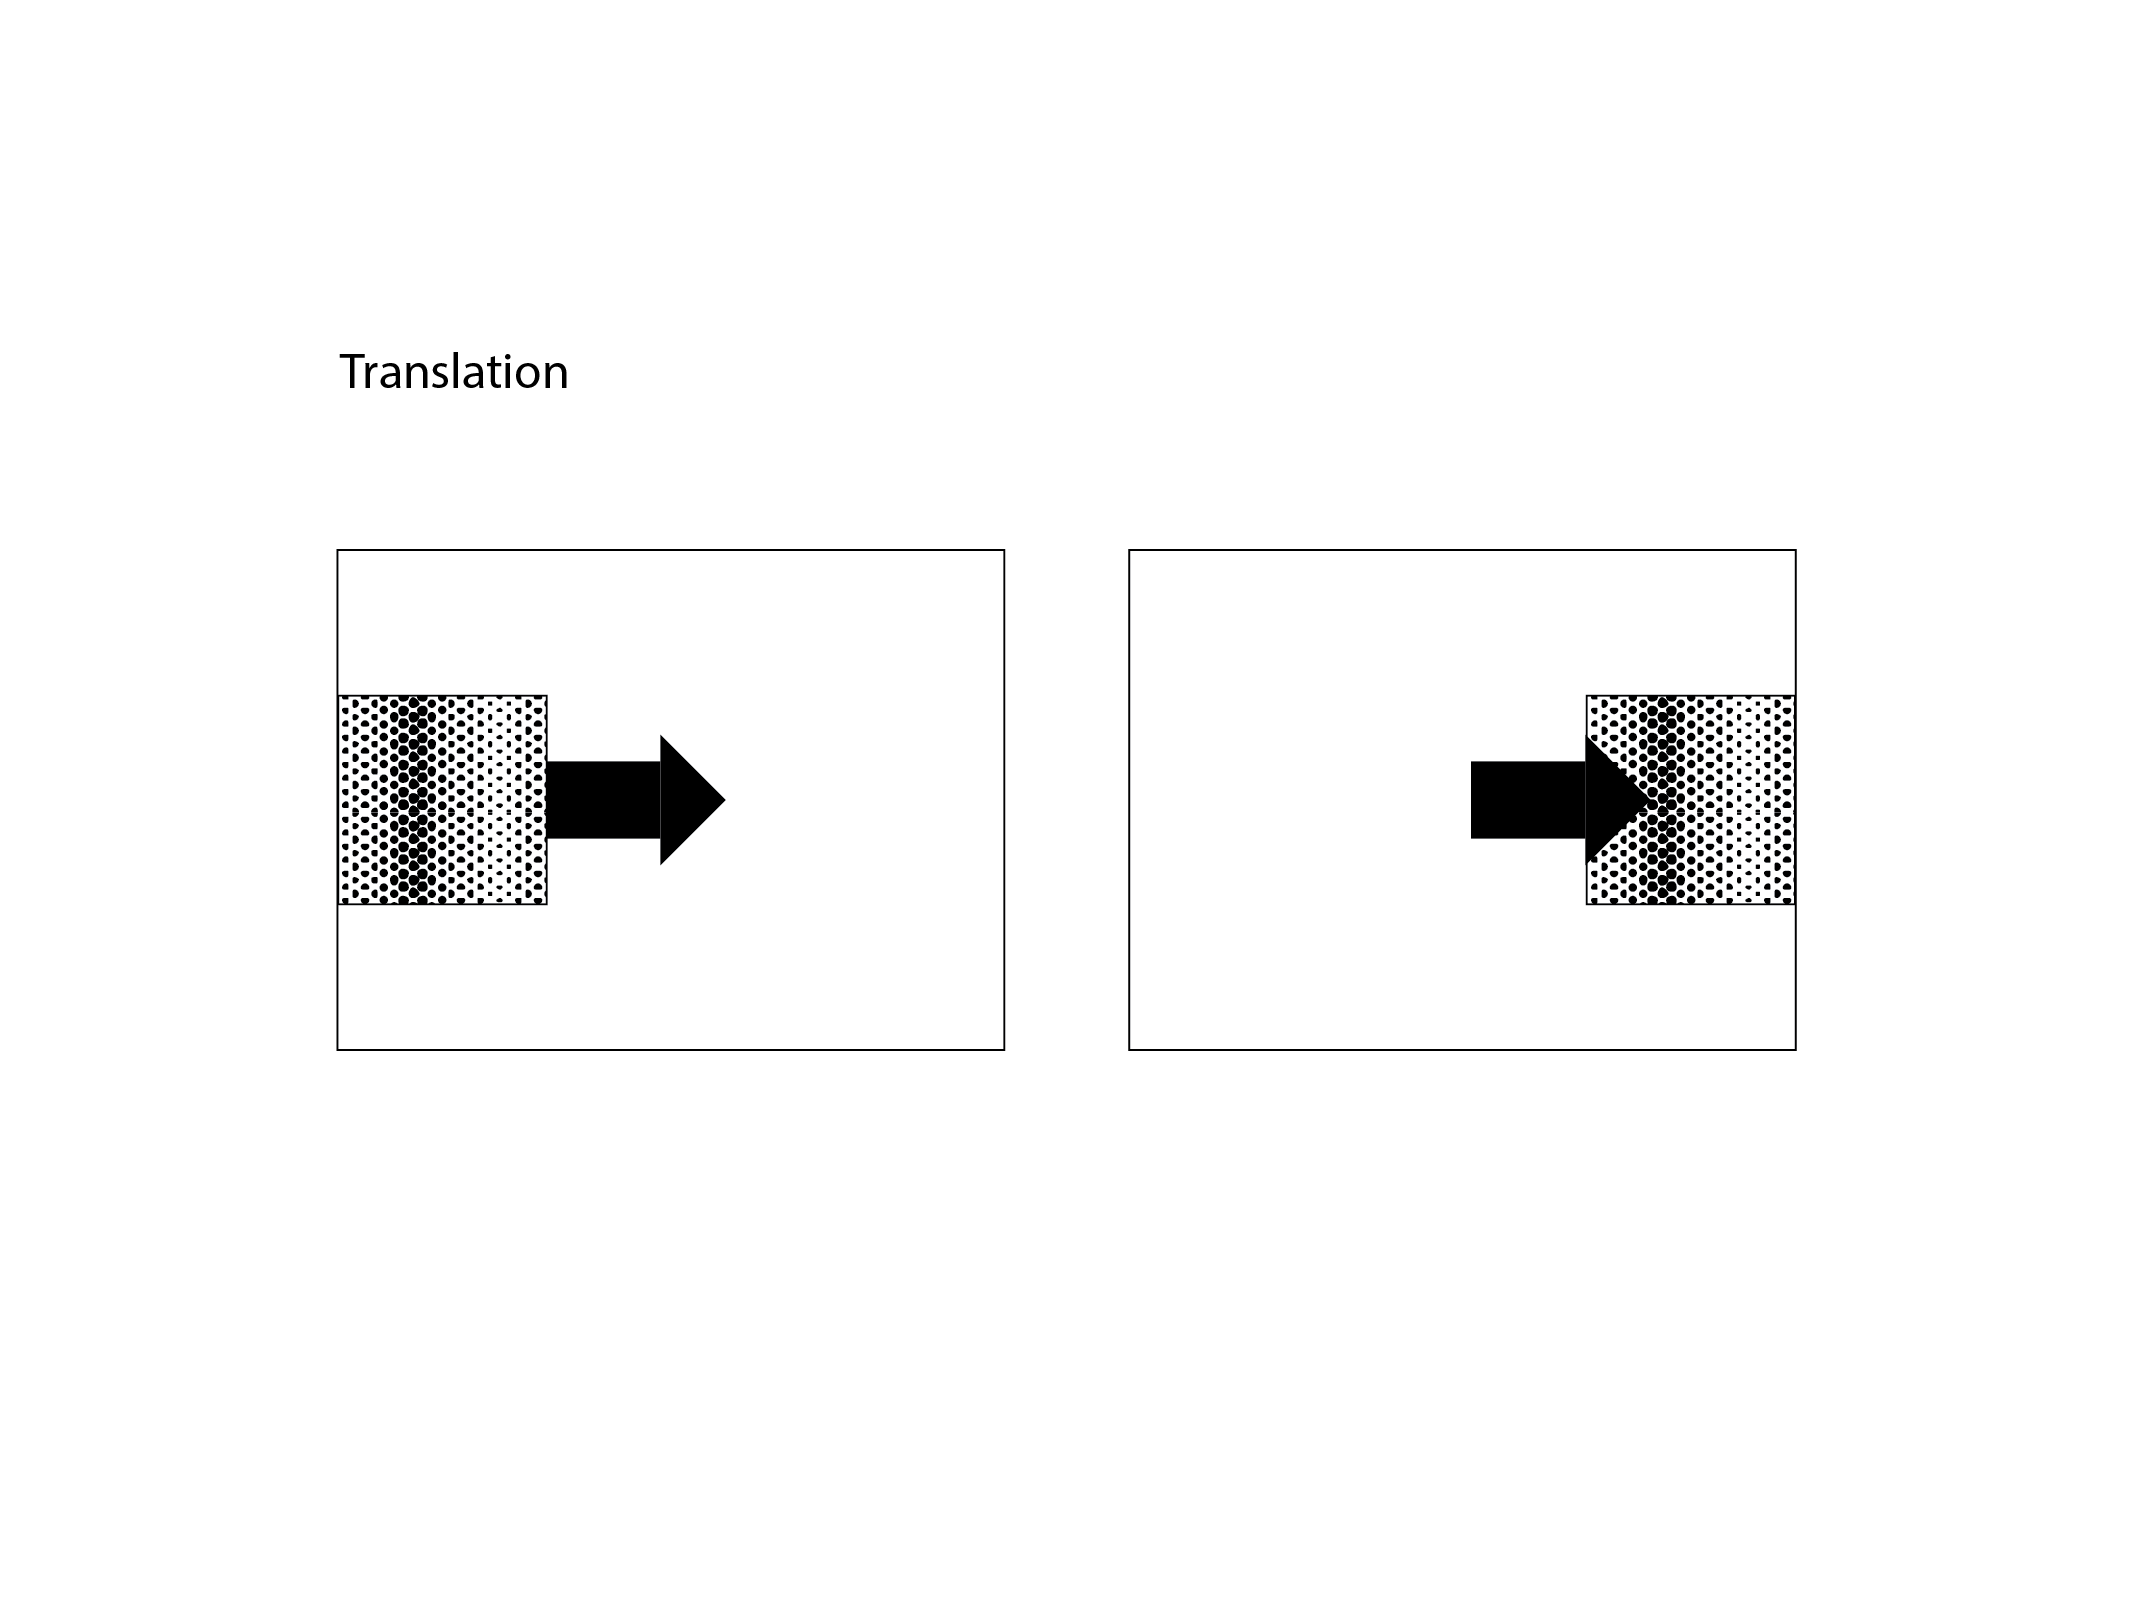
\includegraphics[width=0.75\textwidth]{opticflow_diagrams-01.png}
    \caption{Pattern designed to exploit optic flow calculations in the case of translational motion.}
    \label{fig:lieflat}
\end{figure}

\begin{figure}[H]
    \centering
    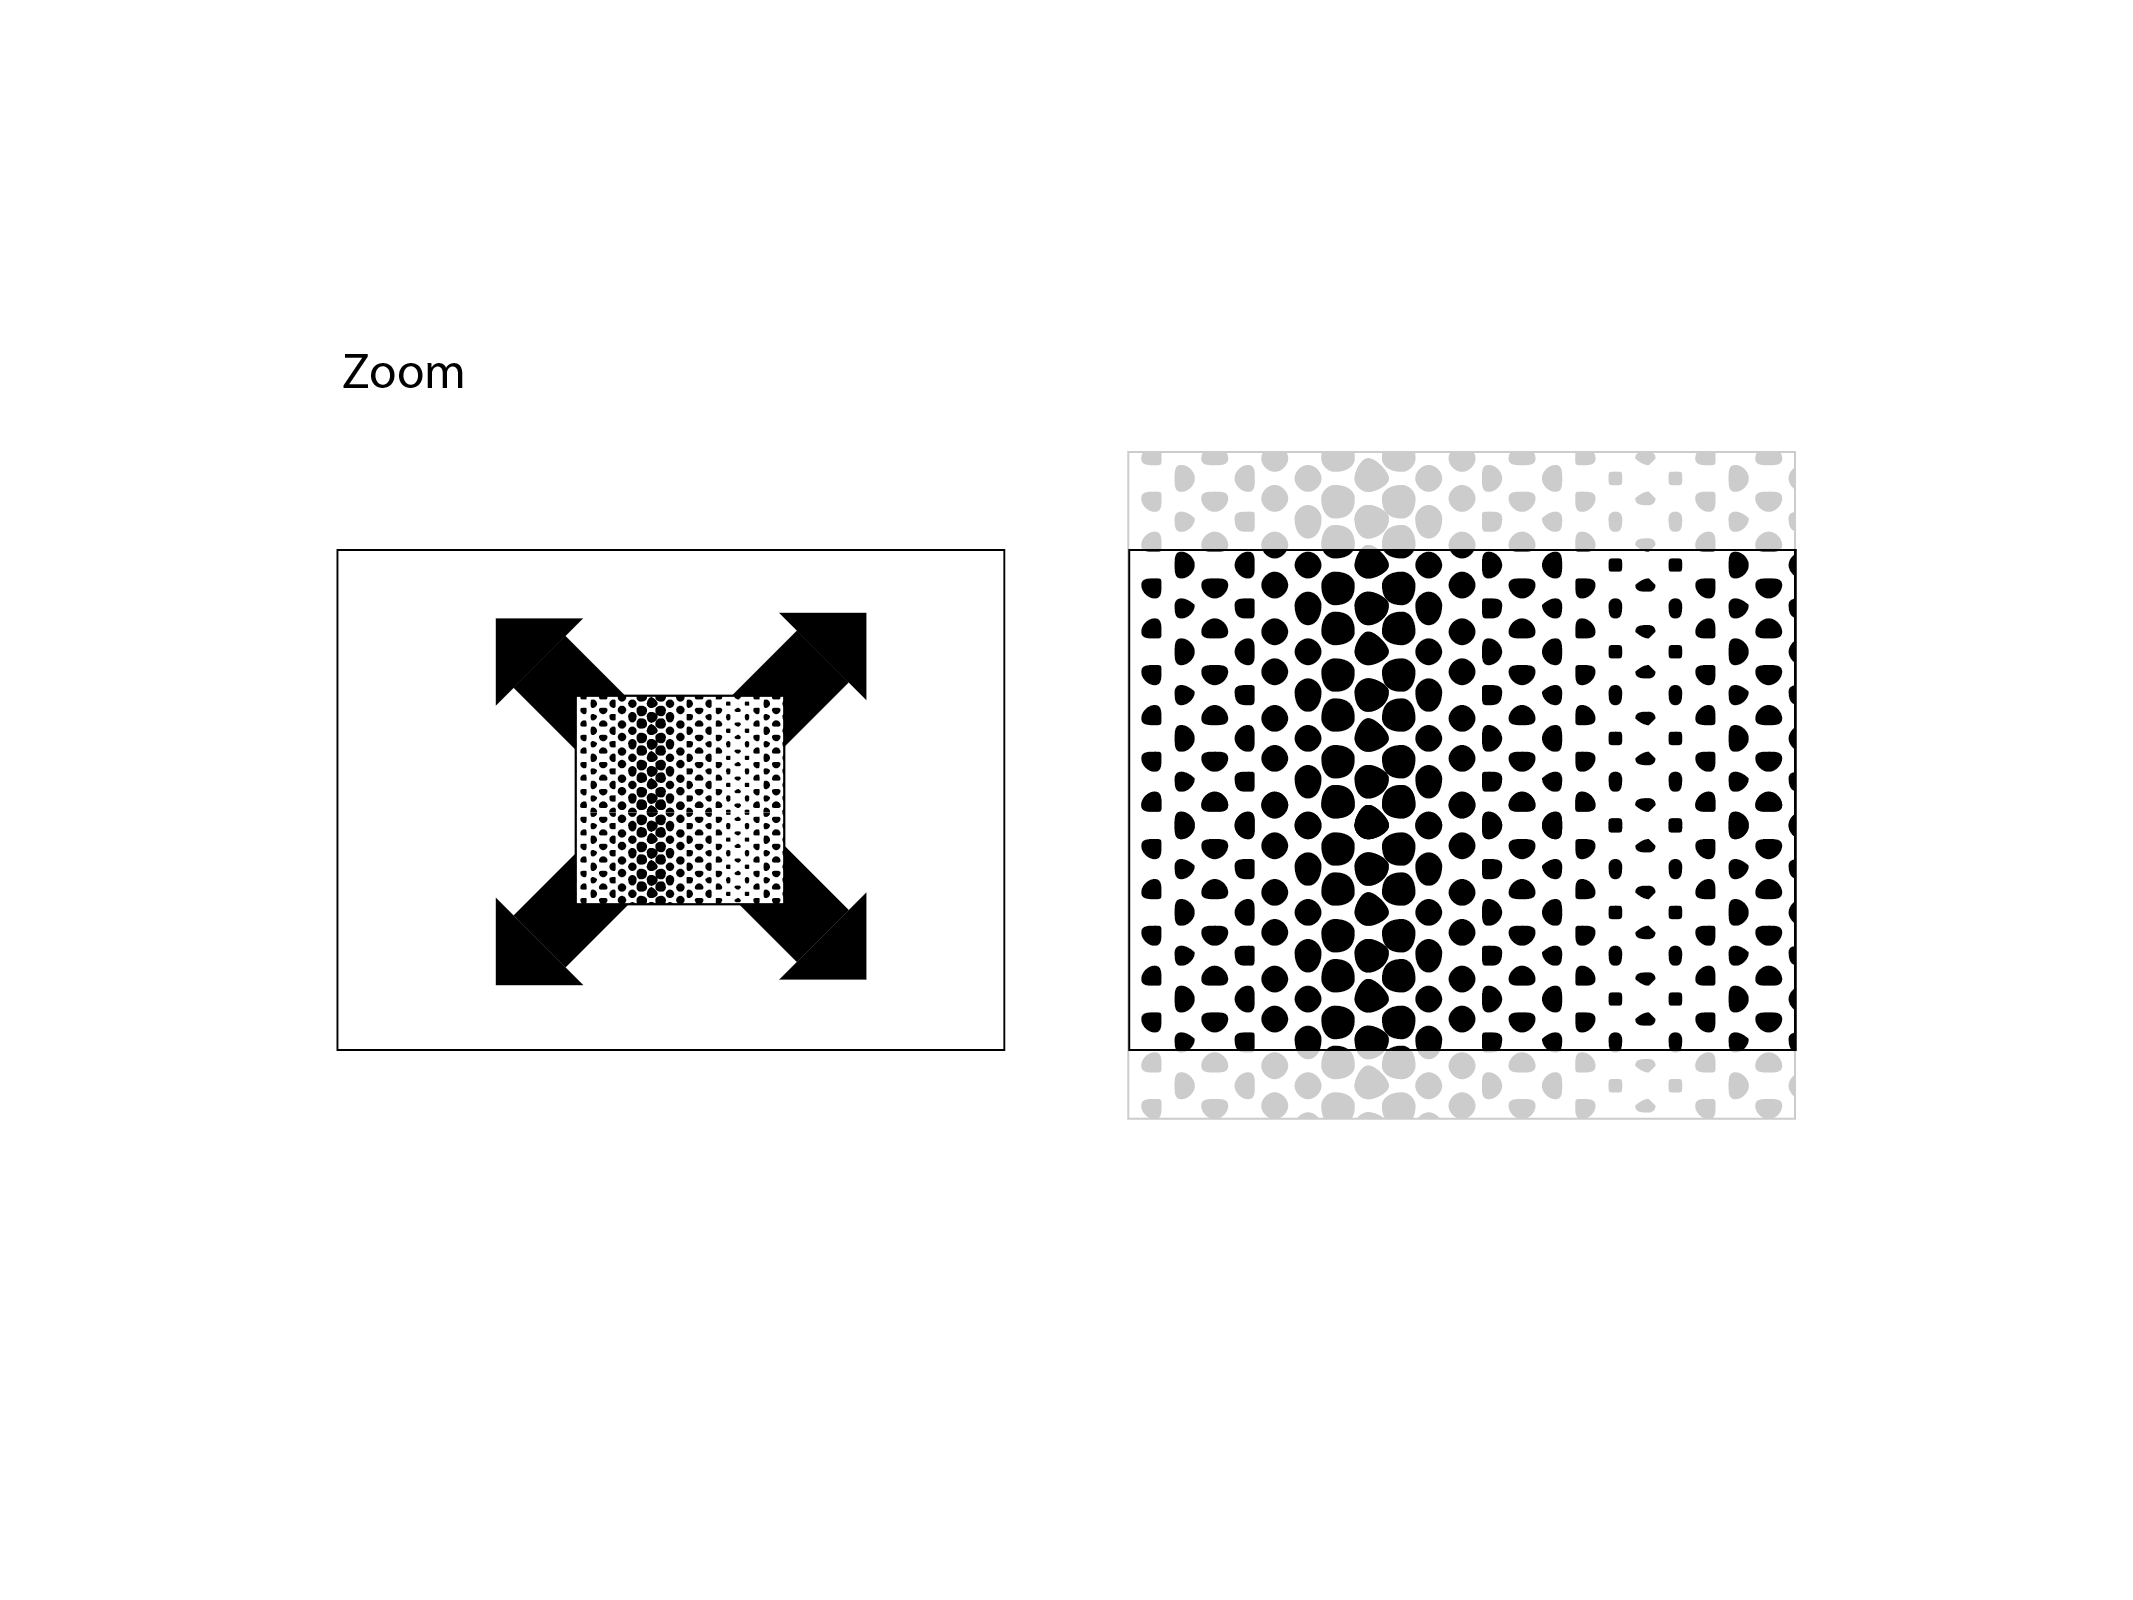
\includegraphics[width=0.75\textwidth]{opticflow_diagrams-02.png}
    \caption{Pattern designed to exploit optic flow calculations in the case of linear motion (or zoom).}
    \label{fig:lieflat}
\end{figure}

\begin{figure}[H]
    \centering
    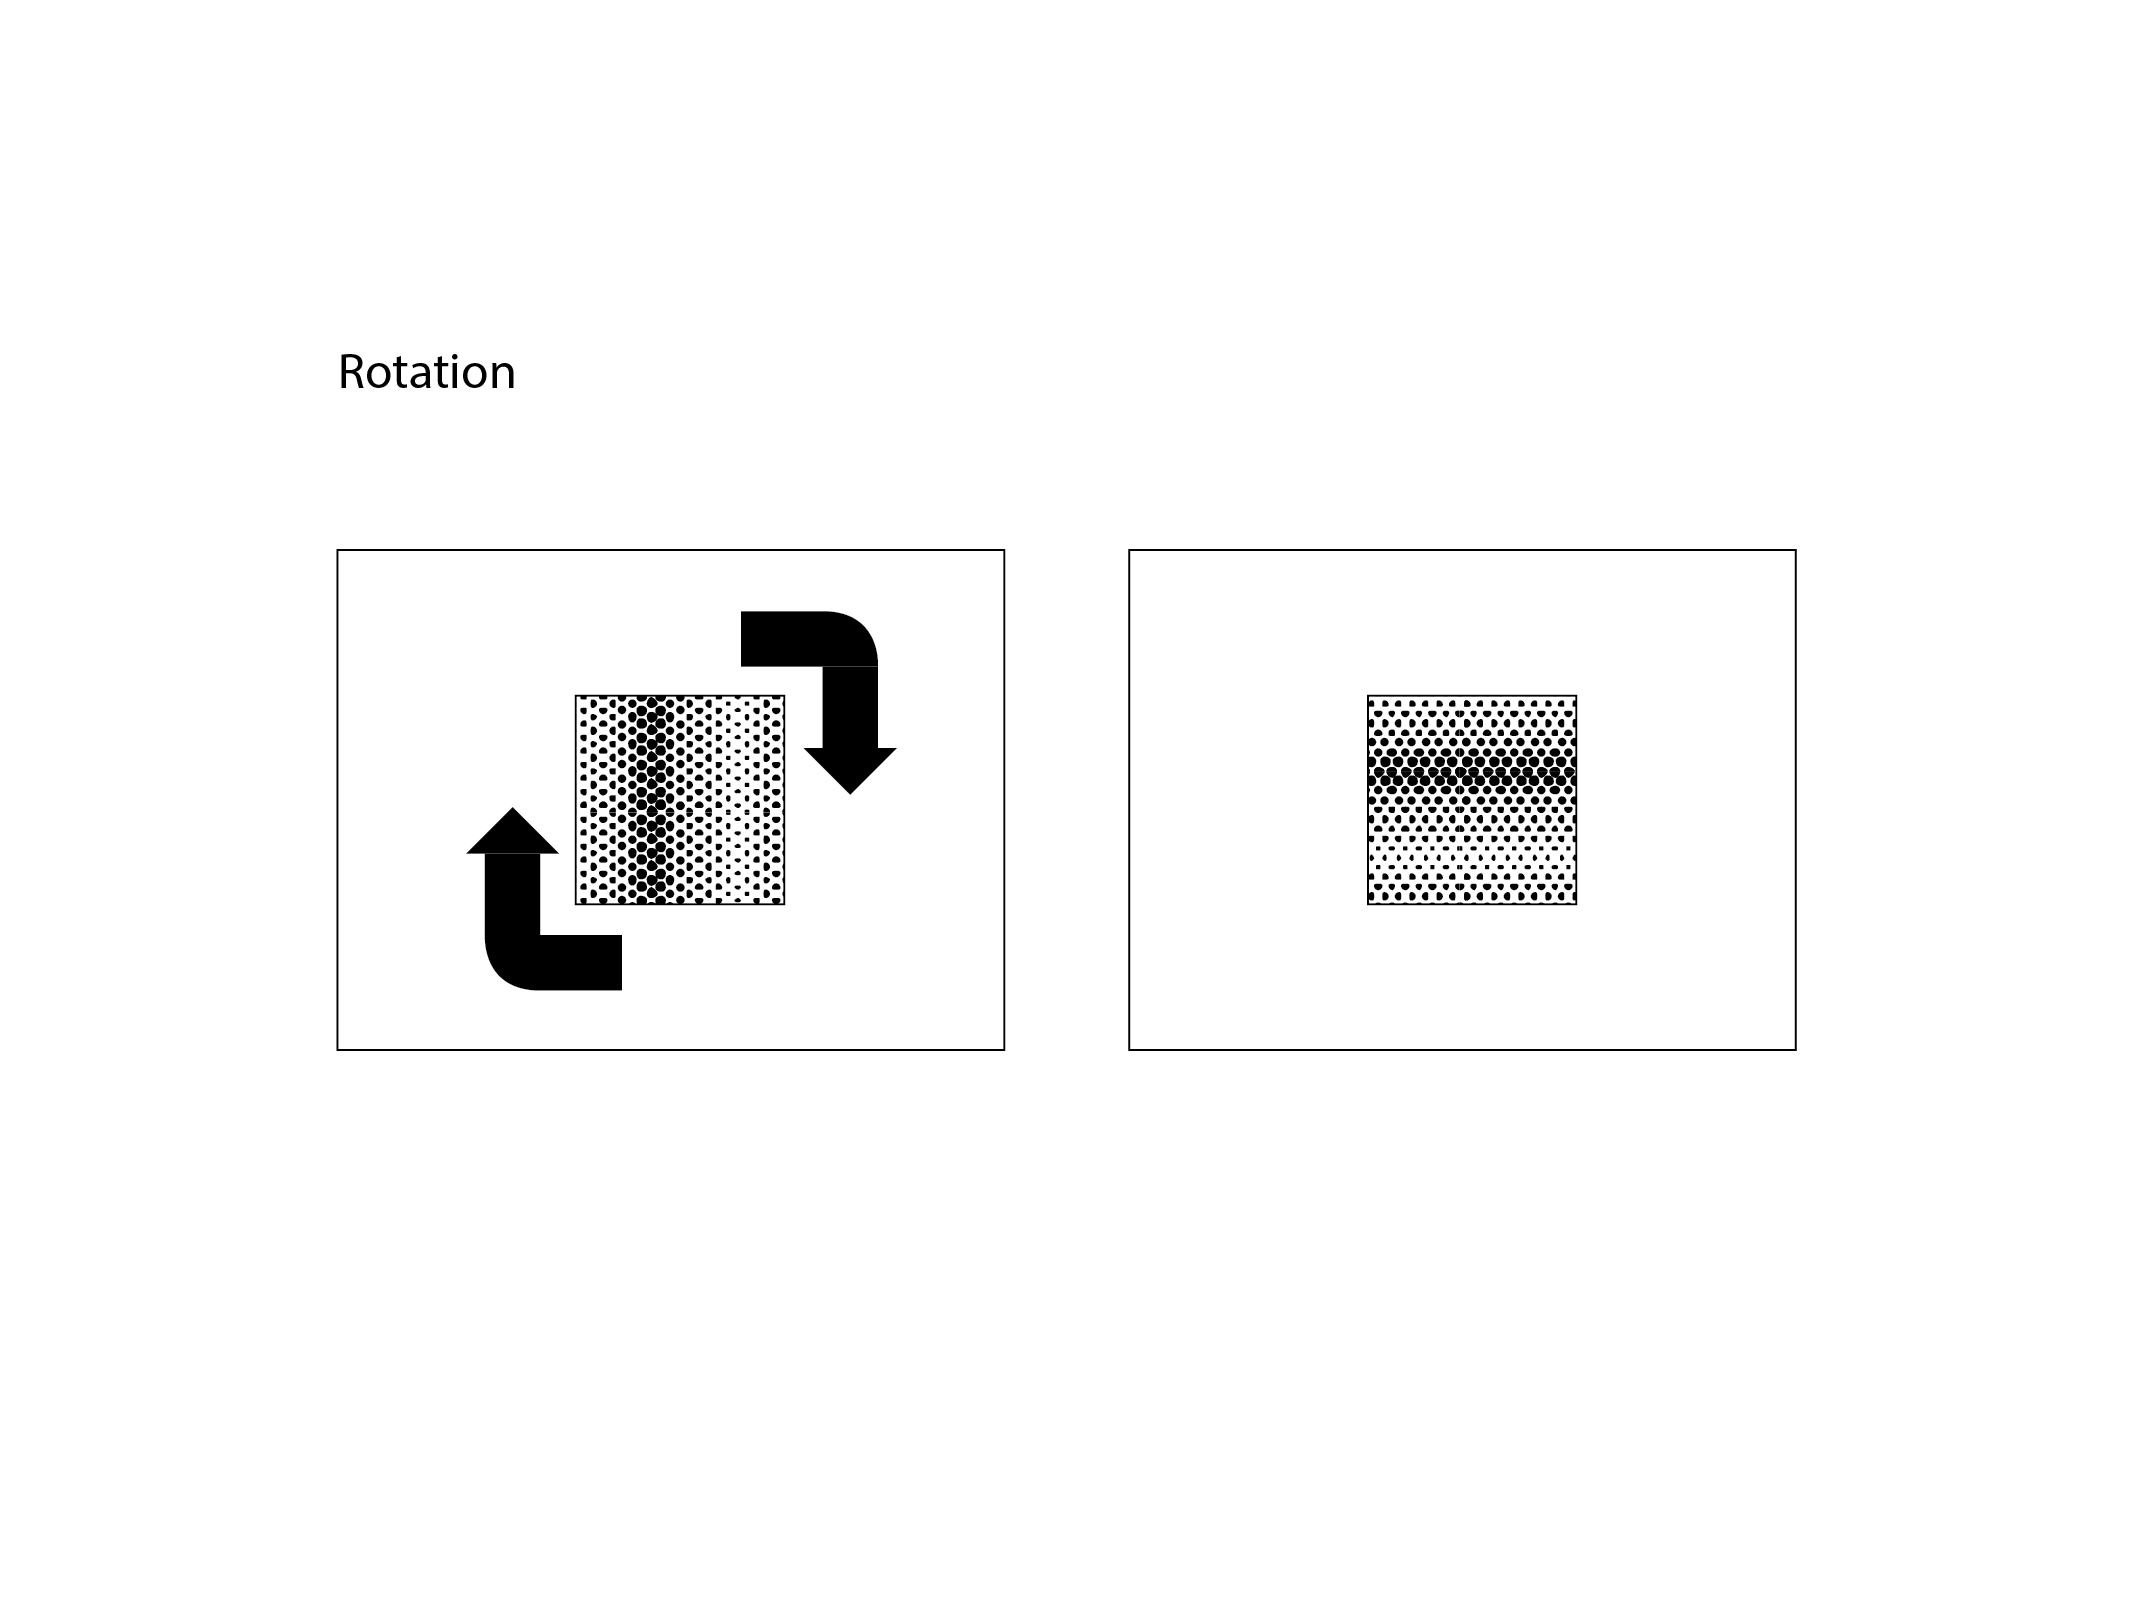
\includegraphics[width=0.75\textwidth]{opticflow_diagrams-03.png}
    \caption{Pattern designed to exploit optic flow calculations in the case of rotational motion.}
    \label{fig:lieflat}
\end{figure}

\vspace{5mm}Once setup, the study will go as follows:

\subsection{Translational Camouflage}
\begin{enumerate}
\item Generate pattern
\item Move pattern from left to right across field of view of virtual camera
\item Fitness test is the amplitude of the collective optic flow perceived by the camera
\item Use crossover and mutation to generate new patterns (using GA)
\item Repeat for n generations (back to step 1)
\end{enumerate} 

\subsection{Approach/Retreat Camouflage}
\begin{enumerate}
\item Generate pattern
\item Move pattern towards virtual camera (zoom)
\item Fitness test is based on a 9 grid set of vectors, looking for inverse vectors mirrored across the center. Success is a resulting vector of magnitude in the opposite direction (i.e. toward perceived, away actual). 
\item Use crossover and mutation to generate new patterns (using GA)
\item Repeat for n generations
\end{enumerate}

\subsection{Rotational Camouflage}
\begin{enumerate}
\item Generate pattern
\item Rotate pattern clockwise in field of view of virtual camera
\item Fitness test is the angular velocity perceived by the camera
\item Use crossover and mutation to generate new patterns (using GA)
\item Repeat for n generations
\end{enumerate}

Some existing examples of this rotational camouflage as a form of of visual deception are the wagon wheel effect, alternately known as a mismatched framerate. This effect is evident in scenarios such as when trying to take video of an airplane's propeller, a different motion is revealed instead of the eye's perceived true motion. Similarly, moire patterns rely on interference or a resolution mismatch to create a more dominant visible pattern. Using these examples as a basis for our approach, our algorithm will look to take advantage of missed frames and antialiasing standard in 30-240fps cameras.

\begin{table}[H]
\begin{tabular}{|p{0.1\textwidth} | p{0.9\textwidth}|}
\hline
	\textbf{Date} & \textbf{Goals} \\
\hline
Tue, 3/31 & \begin{itemize} \item Project Proposal hand in                                                                                                                                                                                                                                                                                                                                                                                                                                                                                                                                                                                                                                                                                                                                                                                       \end{itemize} \\
\hline
Sat, 4/11 & \begin{itemize} \item Prototype of camouflage pattern generation through evolutionary algorithm verified against a fitness function using optic flow calculations. \item Construct scenarios which we can hand-design; aim to evolve expected results. \item Full frame pattern to mitigate concerns with regard to edge detection in optic flow computation. Run computation of camouflage pattern on these scenarios. \item Create GUI for result verification. \item Authors should be comfortable with all tools to be used in project: DEAP evolutionary algorithm package, OpenCV for optic flow calculation and image manipulation. \item Serena lead on using DEAP, Jonathan lead on using OpenCV. Jacob participates in both, preps for hardware testing. \item Following weeks assume success criterion. \end{itemize} \\ \hline
Sat, 4/25 &\begin{itemize} \item Introduce the dilemma of edge detection: instead of having our pattern work only when full-frame, hope to generalize to (a) random backgrounds or (b) selected real-world applicable backgrounds e.g. desert sand, traffic camera. \item Run simultaneous computations using AWS or SEAS computing cluster for a variety of scenarios to test the robustness of camouflage pattern generation. \item Serena and Jonathan break up cases, iterations, and work on this. \item Assuming success criterion, set up a physical testing station using a webcam in place of a camera simulation. \item Test for robustness against aliasing and motion blur. \item Jacob lead on hardware testing.  \item Prepare class presentation of results so far.       \end{itemize}                                                  \\ \hline
Wed, 5/6  & \begin{itemize} \item Prepare final results, write final paper.                                                                                                                                                                                                                                                                                                                                                                                                                                                                                                                                                                                                                                                                                                                                                                                           \end{itemize}  \\ \hline
\end{tabular}
\end{table}

\section{References} 

\setlength\parindent{1cm}

\indent Baird E, Kornfeldt T, Dack M (2010) Minimum viewing angle for visually guided ground speed control in bumblebees. Journal of Experimental Biology  213:1625-1632.\\

Baird E, Srinivasan MV, Zhang SW, Cowling A (2005) Visual control of flight speed in honeybees. Journal of Experimental Biology  208: 3895-3905. \\

Barrows GL, Chahl J, Srinivasan MV (2003) Biologically inspired visual sensing and flight control. Aeronautical Journal  107:159-168. \\

Boedeker N, Kern R, Egelhaaf M (2003) Chasing a dummy target: Smooth pursuit and velocity control in male blowflies. Proceedings of the Royal Society B  270: 393-399.\\

Borst A (2009) Drosophila’s view on insect vision. Current Biology  19: R36-R47.\\

Chahl JS, Srinivasan MV, Zhang SW (2004) Landing strategies in honeybees and applications to uninhabited airborne vehicles. International Journal of Robotics Research  23:101-110. \\

Chahl JS, Srinivasan MV (1996) Visual computation of egomotion using an image interpolation technique. Biological Cybernetics  74: 405-411.\\

Collet TS, Land MF (1978) How hoverflies compute interception courses. Journal of Comparative Physiology  125: 191-204.\\

Collet TS, Land MF (1975) Visual control of flight behaviour in the hoverfly Syritta pipiens. Journal of Comparative Physiology  99:1-66.\\

Dyhr JP, Higgins CM (2010) The spatial-frequency tuning of optic-flow-dependent behaviors in the bumblebee Bombus impatiens. Journal of Experimental Biology  213: 1643-1650.\\

Egelhaaf M (2008) Fly vision: Neural mechanisms of motion computation. International Review of Neurobiology  44: R339-R341.\\

Floreano D, Zufferey JC, Srinivasan MV, Ellington C (2009) Flying insects and robots. Berlin, Heidelberg: Springer 2009.\\

Garratt MA, Chahl JS (2008) Vision-based terrain following for an unmanned aircraft. Journal of Field Robotics  25:284:301. \\

Humbert JS, Hyslop AM (2010) Bioinspired visuomotor convergence. IEEE Transactions on Robotics  26: 121-130.\\

Joesch M, Plett J, Borst A and Reiff DF (2008) Response properties of motion-sensitive visual interneurons in the lobula plate of Drosophila melanogaster. Current Biology  18: 368-374.\\

Land MF, Collett TS (1974) Chasing behaviour of houseflies (Fannia canicularis): A description and analysis. Journal of Comparative Physiology  89: 331-357.\\

Mizutani A, Chahl JS, Srinivasan MV (2003) Motion camouflage in dragonflies. Nature  423:604-1604.\\

Nguyen A, Yosinski J, Clune J (2015) Deep neural networks are easily fooled: High confidence predictions for unrecognizable images. IEEE Computer Vision and Pattern Recognition.\\

Nourani-Vatani N, Roberts J, Srinivasan MV (2009) Practical visual odometry for car-like vehicles. IEEE International Conference on Robotics and Automation. Kobe, Japan. \\

Olberg RM, Worthington AH, Veator KR (2000) Prey pursuit and interception in dragonflies. Journal of Comparative Physiology A  186: 155-162.\\

Ragulskis M, Aleksa A, Saunoriene L (2007) Improved algorithm for image encryption based on stochastic geometric moiré and its application. Optics communications   273: 370-378.\\

Serres JR, Masson GP, Ruffier F, Franceschini N (2008) A bee in the corridor: Centering and wall-following. Naturwissenschaften  95:1181-1187. \\

Srinivasan MV (2011) Visual control of navigation in insects and its relevance for robotics. Current Opinion in Neurobiology  21: 535-543. \\ 

Srinivasan MV (2011) Honeybees as a model for the study of visually guided flight, navigation and biologically inspired robotics. Physiological Reviews  91: 413-460. \\

Srinivasan M, Thurrowgood S, Soccol D (2009) From flying insects to autonomously navigating robots. IEEE Robotics and Automation Magazine  16: 59-71.\\

Srinivasan MV, Zhang SW, Chahl JS, Barth E, Venkatesh S (2000) How honeybees make grazing landings on flat surfaces. Biological Cybernetics  83: 171-183.\\

Tammero LF, Dickinson MH (2002) The influence of visual landscape on the free flight behavior of the fruit fly Drosophila melanogaster. Journal of Experimental Biology  205: 327-343.\\

Weber K, Venkatesh S, Srinivasan MV (1997) Insect inspired behaviors for the autonomous control of mobile robots. In Living From Living Eyes to SEeing Machines. Oxford University Press. \\


Srinivasan MV, Davey M (2003) Strategies for active camouflage of motion. Proceedings of the Royal Society B  259:19-25. \\


\end{document}
